\documentclass[12pt, letterpaper]{article}
\usepackage{tikz}
\usetikzlibrary{arrows,positioning,fit,shapes,calc,decorations.pathreplacing,snakes}

\begin{document}

Figure \ref{diffFig} is a diagram that outlines the fundamentals of diffraction and interference of light through a crystal lattice. As seen in the figure, light that reflects of with the incidence with respect to the normal as used in optics).

\begin{figure}[ht!]
\centering
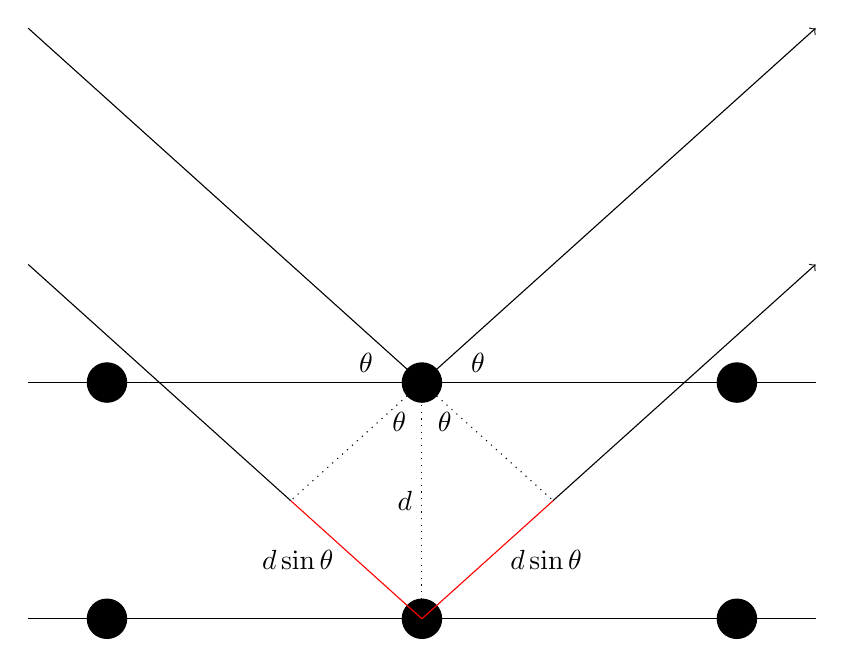
\begin{tikzpicture}[scale=0.5]
    \begin{scope} % Lattice structure
        \draw (0,0) -- ++(20,0);
        \draw (0,6)  --  ++(20,0);
        % Distances
        \draw [dotted](10,0) -- (10,6) node[midway,left]{$d$};
        \draw [dotted](10,6) -- (6.667,3);
        \draw [dotted](10,6) -- (13.333,3);
    \end{scope}
    \begin{scope} % Atoms in lattice
        \foreach \x in {2, 10,  18} \filldraw (\x, 6) circle (.5);
         \foreach \x in {2, 10,  18} \filldraw (\x, 0) circle (.5);
    \end{scope}
    \begin{scope} % Draw light rays
        \draw[->](0,15) -- (10,6) -- (20,15); % Ray reflecting from top layer
    	\draw[-](0,9) -- (6.667,3); % Incoming part of ray reflecting form bottom layer
    	\draw[->](13.33,3) -- (20,9); % Outgoing part of ray reflecting from botton layer
    \end{scope}

% Angles at appropriate places
\coordinate (t1) at (9,6.5);
\node[left] at (t1) {$\theta$};
\coordinate (t3) at (11,6.5);
\node[right] at (t3) {$\theta$};
\coordinate (t2) at (9,5);
\node[right] at (t2) {$\theta$};
\coordinate (t4) at (11,5);
\node[left] at (t4) {$\theta$};

% Mark the path difference with red and add equation for extra path distance traveled by ``second'' ray
\coordinate (pL1) at (8,1.5);
\node[left] at (pL1) {$d\sin\theta$};
\draw [-,red](6.667,3) --(10,0);
\coordinate (pL2) at (12,1.5);
\node[right] at (pL2) {$d\sin\theta$};
\draw [-,red](10,0) --(13.333,3);

\end{tikzpicture}% Fin :P
\caption{Diffraction of X-rays by a crystal lattice.}\label{diffFig}
\end{figure}




\begin{figure}[ht!]
\centering
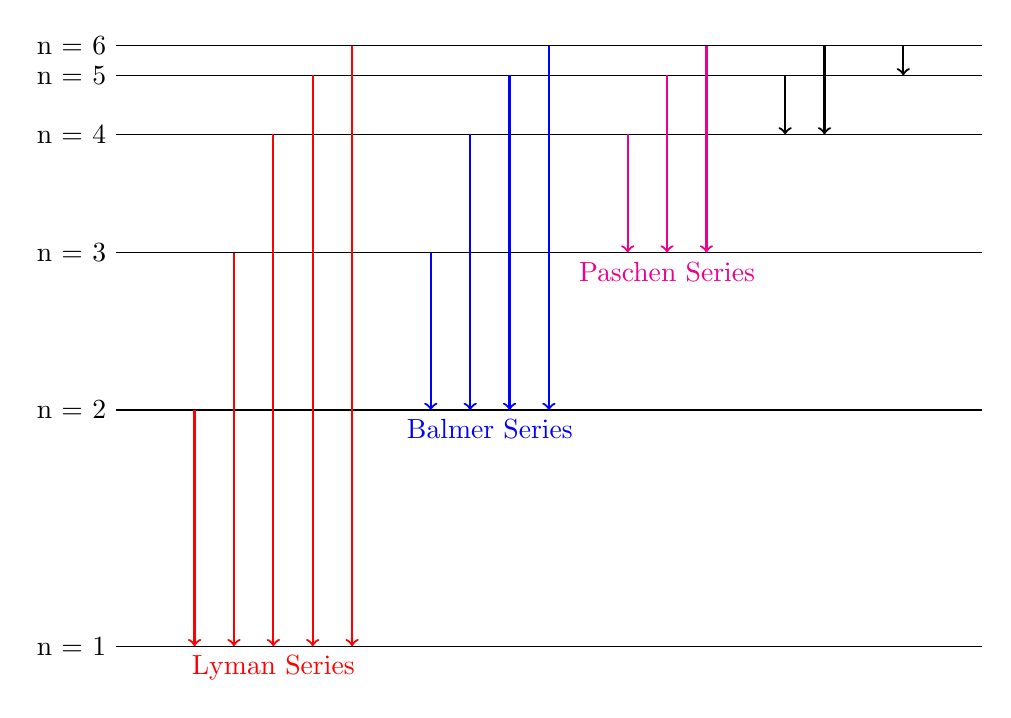
\begin{tikzpicture}[scale=0.5]

\coordinate (L) at (4,0);
\node[below,red] at (L) {Lyman Series};
\coordinate (B) at (9.5,6);
\node[below,blue] at (B) {Balmer Series};
\coordinate (P) at (14,10);
\node[below,magenta] at (P) {Paschen Series};


\coordinate (n1) at (0,0);
\node[left] at (n1) {n = 1};
\coordinate (n2) at (0,6);
\node[left] at (n2) {n = 2};
\coordinate (n3) at (0,10);
\node[left] at (n3) {n = 3};

\coordinate (n4) at (0,13);
\node[left] at (n4) {n = 4};
\coordinate (n5) at (0,14.5);
\node[left] at (n5) {n = 5};
\coordinate (n6) at (0,15.25);
\node[left] at (n6) {n = 6};


    \begin{scope} % Energy levels
        \draw (0,0)   --  (22,0);
        \draw (0,6)   --  (22,6);
        \draw (0,10)  --  (22,10);
        \draw (0,13)  --  (22,13);
        \draw (0,14.5)  --  (22,14.5);
        \draw (0,15.25)  --  (22,15.25);
    \end{scope}

    \begin{scope} % Dropping electrons
    	\draw [->, thick,red](2,6) -- (2,0);
        \draw [->, thick,red](3,10) -- (3,0);
        \draw [->, thick,red](4,13) -- (4,0);
        \draw [->, thick,red](5,14.5) -- (5,0);
        \draw [->, thick,red](6,15.25) -- (6,0);
        \draw [->, thick,blue](8,10) -- (8,6);
        \draw [->, thick,blue](9,13) -- (9,6);
        \draw [->, thick,blue](10,14.5) -- (10,6);
        \draw [->, thick,blue](11,15.25) -- (11,6);
        \draw [->, thick,magenta](13,13) -- (13,10);
        \draw [->, thick,magenta](14,14.5) -- (14,10);
        \draw [->, thick,magenta](15,15.25) -- (15,10);
        \draw [->, thick](17,14.5) -- (17,13);
        \draw [->, thick](18,15.25) -- (18,13);
        \draw [->, thick](20,15.25) -- (20,14.5);
	\end{scope}


    \end{tikzpicture}
\caption{Energy level diagram for the hydrogen atom.}\label{hydrogenELevels}
\end{figure}




\begin{figure}[ht!]
\centering
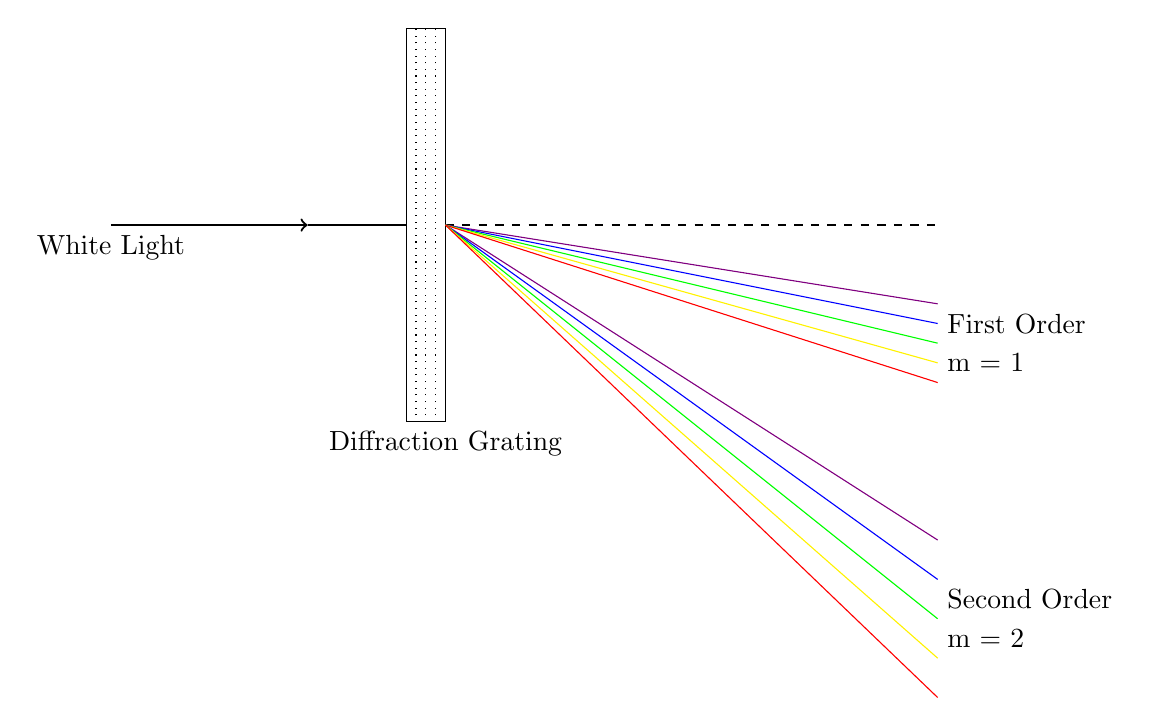
\begin{tikzpicture}[scale=0.5]
	\begin{scope} % Incoming light
		\draw[->,thick]node[below]{White Light} (0,0)-- (5,0);
		\draw[-,thick](5,0) -- (7.5,0);
		\draw[dashed,thick](8.5,0) -- (21,0);
	\end{scope}

	\begin{scope}% Diffraction Grating
		\draw[-](7.5,-5) -- (7.5,5)--(8.5,5) -- (8.5,-5)node[below]{Diffraction Grating} -- (7.5, -5);
		\draw[dotted](8,-5) -- (8,5);
		\draw[dotted](8.25,-5) -- (8.25,5);
		\draw[dotted](7.75,-5) -- (7.75,5);
	\end{scope}

	\begin{scope} % First order m = 1
		\draw[-,violet](8.5,0) -- (21,-2);
		\draw[-,blue](8.5,0) -- (21,-2.5);
		\draw[-,green](8.5,0) -- (21,-3);
		\draw[-,yellow](8.5,0) -- (21,-3.5);
		\draw[-,red](8.5,0) -- (21,-4);
	\end{scope}

\coordinate (m11) at (21,-2.5);
\node[right] at (m11) {First Order};
\coordinate (m12) at (21,-3.5);
\node[right] at (m12) {m = 1};

	\begin{scope} % Second order m = 2
		\draw[-,violet](8.5,0) -- (21,-8);
		\draw[-,blue](8.5,0) -- (21,-9);
		\draw[-,green](8.5,0) -- (21,-10);
		\draw[-,yellow](8.5,0) -- (21,-11);
		\draw[-,red](8.5,0) -- (21,-12);
	\end{scope}
\coordinate (m21) at (21,-9.5);
\node[right] at (m21) {Second Order};
\coordinate (m22) at (21,-10.5);
\node[right] at (m22) {m = 2};
\end{tikzpicture}
\caption{Diffraction of light though a grating.}\label{diffGrating}
\end{figure}



\end{document}
